% Figure 3: Claw-N Tensor Accelerator
\documentclass[tikz,border=10pt]{standalone}
\usepackage{tikz}
\usetikzlibrary{arrows.meta,positioning,shapes,calc,fit,backgrounds}

\begin{document}
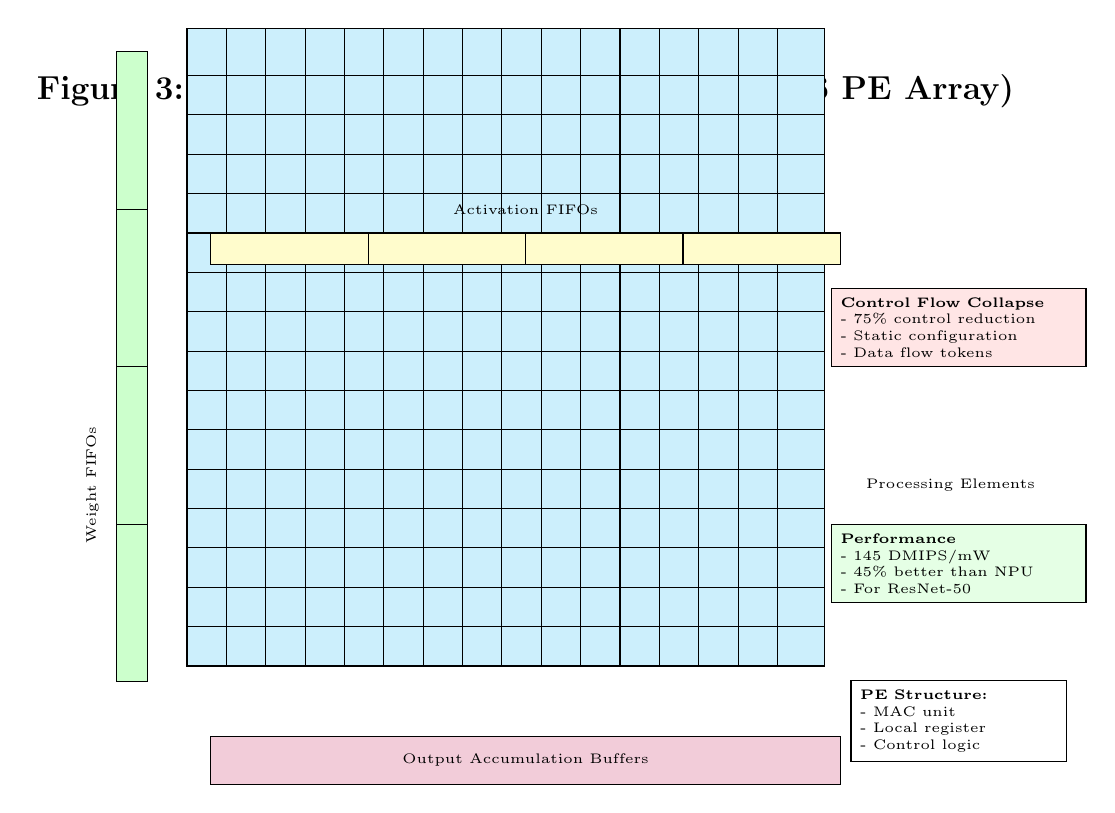
\begin{tikzpicture}[
    node distance=0.5cm,
    pe/.style={rectangle, draw, fill=cyan!20, minimum width=0.6cm, minimum height=0.6cm, font=\tiny},
    arrow/.style={-{Stealth[length=1.5mm]}, thick}
]

% Title
\node[font=\large\bfseries] at (0,5) {Figure 3: Claw-N Tensor Accelerator (16$\\times$16 PE Array)};

% PE Array
\foreach \i in {0,...,15} {
    \foreach \j in {0,...,15} {
        \node[pe] (pe\i\j) at (\i*0.5-4, \j*0.5-2) {};
    }
}

% Label PEs
\node[font=\tiny, right] at (4.2,0) {Processing Elements};

% Weight FIFOs (left)
\foreach \j in {0,4,8,12} {
    \node[rectangle, draw, fill=green!20, minimum width=0.4cm, minimum height=2cm] at (-5, \j*0.5-1.5) {};
}
\node[font=\tiny, rotate=90] at (-5.5,0) {Weight FIFOs};

% Activation FIFOs (top)
\foreach \i in {0,4,8,12} {
    \node[rectangle, draw, fill=yellow!20, minimum width=2cm, minimum height=0.4cm] at (\i*0.5-3, 3) {};
}
\node[font=\tiny] at (0,3.5) {Activation FIFOs};

% Output buffers (bottom)
\node[rectangle, draw, fill=purple!20, minimum width=8cm, minimum height=0.6cm] at (0,-3.5) {};
\node[font=\tiny] at (0,-3.5) {Output Accumulation Buffers};

% Control Flow Collapse annotation
\node[draw, fill=red!10, align=left, font=\tiny, text width=3cm] at (5.5,2) {
    \textbf{Control Flow Collapse}\\
    - 75\% control reduction\\
    - Static configuration\\
    - Data flow tokens
};

% Energy efficiency annotation
\node[draw, fill=green!10, align=left, font=\tiny, text width=3cm] at (5.5,-1) {
    \textbf{Performance}\\
    - 145 DMIPS/mW\\
    - 45\% better than NPU\\
    - For ResNet-50
};

% PE detail
\node[draw, fill=white, font=\tiny, align=left, text width=2.5cm] at (5.5,-3) {
    \textbf{PE Structure:}\\
    - MAC unit\\
    - Local register\\
    - Control logic
};

\end{tikzpicture}
\end{document}
